\documentclass[11pt, class=article, crop=false]{standalone}
\usepackage{amsmath,amssymb,amsfonts,amsthm}
\usepackage{enumitem}
\usepackage{fancyhdr}
\usepackage{tikz-cd}
\usepackage{mathabx}
\usepackage{geometry}
\usepackage{color}
\usepackage{natbib}
\usepackage{braket}
\usepackage{graphicx}
\usepackage{hyperref}
\usepackage{listings}
\usepackage{kiritsis}
\geometry{margin = 0.5in}

\begin{document}
	\section*{Chapter 2: Classical String Theory} % (fold)
	\label{sec:chapter_2_classical_string_theory}
	\begin{enumerate}
		\item I don't know what this question asks exactly given that 2.1.16 is an infinitesimal diffeomorphism.  
		
		 We are still allowed to assume WLOG that $\tau$ runs from $0$ to $1$. For $\xi$ infinitesimal, we have $\delta e = \xi \dot e + \dot \xi e = \partial_\tau (\xi e)$. So for a general $e(\tau)$ define
		\begin{equation}
			\tau_2(\tau) = \frac{\int_0^\tau d\tau' e(\tau') }{\int_0^1 d\tau' e(\tau')}
		\end{equation} 
		Take $L = \int_0^1 d\tau' e(\tau')$. Then $e_2(\tau_2(\tau)) = \left(\frac{d\tau_2}{d\tau}\right)^{-1} e(\tau) = \left( \frac{e(\tau)}{L} \right)^{-1} e(\tau) = L$.
		
		Note that we cannot get rid of this $L$, since it is invariant $L = \int_0^1 d\tau e(\tau) = \int_0^1 d\tau_2 e(\tau_2)$
		
		
		\item From analytic continuation, we have the functional equation for the Riemann zeta function:
		\begin{equation}
			\zeta(s) = 2^s \pi^{s-1} \sin(\frac{\pi s}{2}) \Gamma(1-s) \zeta(1-s)
		\end{equation}
		It is worth knowing that near $s=0$ we have $\zeta(1-s) = -\frac{1}{s} + \gamma$ and $\Gamma(1-s) = 1 + \gamma s$. Expanding the right hand side about $s = 0$ gives
		\begin{equation}
			\zeta(\epsilon) = -\frac12 - \frac12 \sqrt{2 \pi} \epsilon
		\end{equation}
		This gives $\zeta(0) = -\frac12$ and $\zeta'(0) = -\frac12 \sqrt{2\pi}$. Further, $\zeta'(s) = - \sum_{n=1}^\infty \frac{\log n}{n^s}$. 
		
		So we get $\prod_{n=1}^\infty \frac{1}{L^2} = L^{-2 \sum_{n=1}^\infty 1} = L^{-2 \zeta(0)} = L$ and $\prod_{n=1}^\infty n^2 = \exp\left(2 \sum_{n=1}^\infty \log n \right) = 2\pi$.
		
		\item For simplicity, we will work in the action with the einbein.
		\[
			\frac12 \int d\tau e (e^{-2} G_{\mu \nu} \dot x^\mu \dot x^\nu - m^2) % \to \frac L2 \int d\tau {\frac{G_{\mu \nu} \dot x^\mu \dot x^\nu}{L^2} - m^2}
		\]
		 % We can gauge fix $e$ to $L$.
		The Euler-Lagrange equations for $x^\mu$ is:
		\begin{equation}
			\begin{aligned}
				\frac{d}{d\tau} \frac{\partial}{\partial x^\mu} (e^{-1} G_{\alpha \beta} \dot x^\alpha \dot x^\beta) - \frac{\partial}{\partial x^\mu}\left( e^{-1} G_{\alpha \beta} \dot x^\alpha \dot x^\beta \right)
				&= 2 e^{-1} G_{\mu \nu} \ddot x^\nu + 2 e^{-1} \partial_\gamma G_{\mu \nu} \dot x^\nu \dot x^\gamma - 2 \frac{G_{\mu \nu} \dot x^\nu}{e^2} \dot e  - e^{-1} \partial_\mu G_{\alpha \beta} \dot x^\alpha \dot x^\beta\\
				&\to G_{\mu \nu} \ddot x^\nu + \frac12 (\partial_\gamma G_{\mu \nu} + \partial_\nu G_{\mu \gamma} - \partial_\mu G_{\nu \gamma}) \dot x^\nu \dot x^\gamma - \frac12 G_{\mu \nu} \dot x^\nu \partial_\tau \log e^2 \\
			\end{aligned}
		\end{equation}
		This last term looks particularly annoying, and is ignored by other authors. We have total freedom in reparameterization of $e$, so we can WLOG set it equal to a (metric-dependent) constant by problem $1$. Then the term drops out and we get exactly the geodesic equations. 

		We could have done this explicitly as well: 
		\begin{equation}
			\begin{aligned}
				\frac{d}{d\tau} \frac{G_{\mu \nu} \dot x^\nu}{\sqrt{G_{\alpha \beta} \dot x^\alpha \dot x^\beta}} - \frac{\partial}{\partial x^\mu} \sqrt{G_{\alpha \beta} \dot x^\alpha \dot x^\beta} &= \frac{G_{\mu \nu} \ddot x^\nu + \partial_\lambda G_{\mu \nu} \dot x^\nu \dot x^\lambda - \frac12 \partial_\mu G_{\nu \lambda} \dot x^\nu \dot x^\lambda}{ \sqrt{-G_{\alpha \beta} \dot x^\alpha \dot x^\beta}} + G_{\mu \nu} \dot x^\nu \frac{d}{d\tau} (-G_{\alpha \beta} \dot x^\alpha \dot x^\beta)^{-1/2}\\
				&= G_{\mu \nu} (\ddot x^\nu + \Gamma^\nu_{\alpha \beta} \dot x^\alpha \dot x^\beta) - \frac12 G_{\mu \nu} \dot x^\nu \frac{d}{d\tau} \log(-G_{\alpha \beta} \dot x^\alpha \dot x^\beta)
			\end{aligned}
		\end{equation}
		And fix the parameterization so that $x^2 = \mathrm{const}$ and the last term vanishes.
		
		\item We get the same as before, but now cannot drop the last term. Now the dots represent time derivatives.
		\begin{equation}
			 G_{\mu \nu} (\ddot x^\nu + \Gamma^\nu_{\alpha \beta} \dot x^\alpha \dot x^\beta) - \frac12 G_{\mu \nu} \dot x^\nu \partial_{X^0} \log(-G_{\alpha \beta} \dot x^\alpha \dot x^\beta)
		\end{equation}
		
		\item We get: 
		\begin{equation}
			-m c \int d\tau \sqrt{-(G_{00} \dot x^0 \dot x^0 + 2 G_{0i} \dot x^0 \dot x^i + G_{ij} \dot x^i \dot x^j)}
		\end{equation}
		Taking $\tau = x^0 = ct$ gives us our result. Further, we write $G_{00} = -1 - \frac{2 \phi}{c^2}$ where $\phi$ is the gravitational potential. To first order then we get:
		\begin{equation}
			-m c^2 \int dt \sqrt{-(G_{00} + 2 c^{-1} G_{0i} \dot x^i +  c^{-2} G_{ij} \dot x^i \dot x^j)} \approx  \int dt \left(- m c^2 - m \phi  + m c G_{0 i} v^i +  m G_{ij} v^i v^j\right)
		\end{equation}
		The last two terms in brackets are positive (kinetic) while the first two are negative (potential). \textbf{This explains why there is a - sign out front of the action}.
		
		\begin{center}
			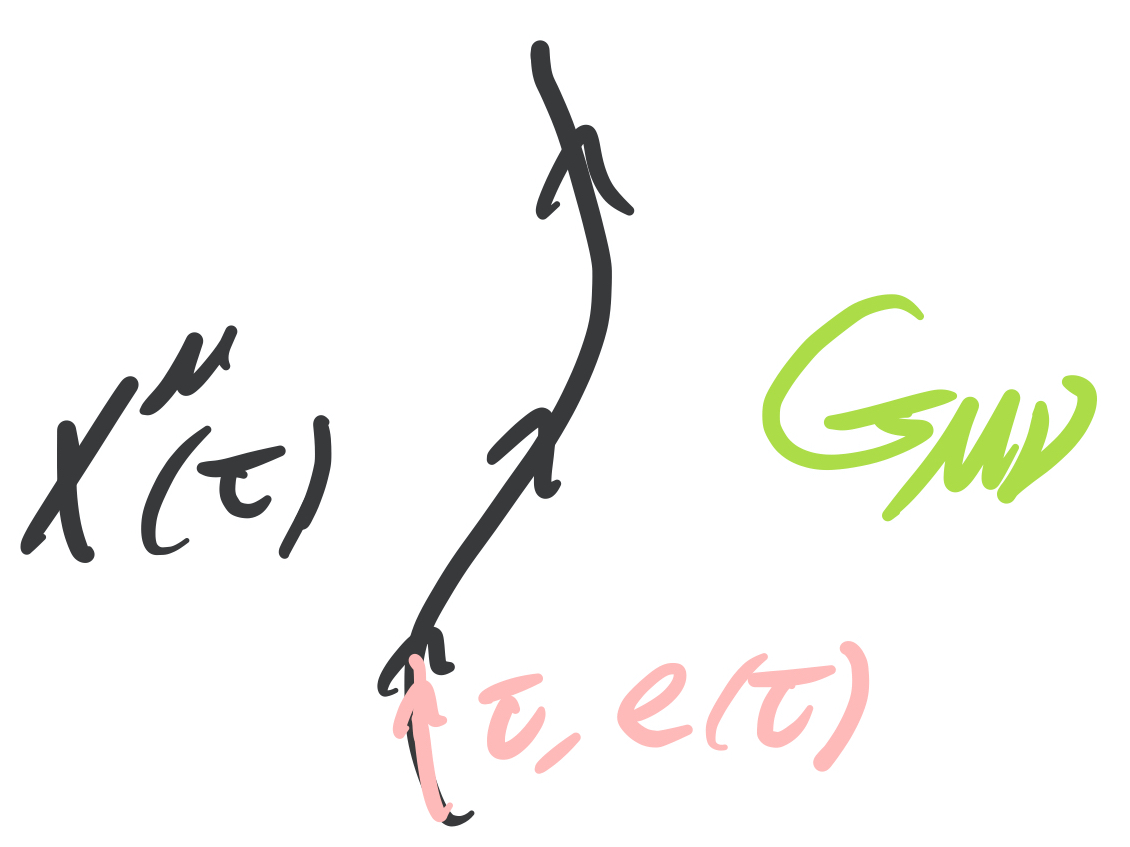
\includegraphics[scale=0.12]{Drawings/Particle}
		\end{center}
		
		\item The Lagrangian for a special relativistic particle in an electromagnetic field is $-mc^2 \sqrt{1-v^2/c^2} - e \phi + e \vec v \cdot \mathbf{A}$. This has the Lorentz invariant form: $-m \sqrt{-G_{\mu \nu} \dot x^\mu \dot x^\nu} + e A_\mu \dot x^\mu$. We get equations of motion as before: 
		The additional term gives the equations of motion:
		\begin{equation}
			\frac{e}{m} (\dot A_\mu - \partial_\mu A_\nu \dot x^\nu) =  \frac{e}{m} (\partial_\nu A_\mu - \partial_\mu A_\nu \dot) x^\nu =  \frac{e}{m} F_{\mu \nu} \dot x^\nu
		\end{equation}
		don't confuse $e$ with the einbein. 
		
		If one coordinate is cyclic (neither the metric nor the vector potential depend on it), the corresponding momentum is 
		\begin{equation}
			\frac{\partial \mathcal L}{\partial \dot x^\mu} = m\frac{G_{\mu \nu} \dot x^\nu}{\sqrt{-G_\mu \nu \dot x^\mu \dot x^\nu}} + e A_\mu
		\end{equation}
		
		\item Ignoring the cosmological constant term (which is not reparameterization invariant), we note that any term that involves the metric $G_{\mu \nu}$ will require at least $2$ $x^\mu$ variables for it to be contracted with. Also, reparameterization invariance requires that under $d\tau \to f'(\tau) d\tau$ we get $\mathcal L \to \mathcal L/\lambda$. The simplest such term is $\sqrt{-G_{\mu \nu} \dot x^\mu \dot x^\nu}$. Terms with more than $2$ $x^\mu$s will be suppressed by powers of $1/\ell_s^2$. Similarly, terms with more derivatives w.r.t. worldsheet coordinates will be less relevant in the IR. 
		
		\item Let's set $G_{i0}=0$ for simplicity. The Nambu-Goto action is:
		\[
			-T \int d\tau d\sigma \sqrt{(\dot X \cdot X')^2 - (\dot X^2) ({X'}^2)} 
		\]
		Take $\tau = c t$, $\sigma = x$ and note $T = \rho c^2$ with $\rho$ the mass per unit length. Take $X^0= ct$ % and $X^1 = x$ so that ${X'}^{0} = 0, \dot X^1 = 0$
		and $\vec u = {X'}^i, \vec v = \dot X^i$. Appreciate that $v$ gives us how that point of the string is moving, while $u$ gives the direction parallel to the string at that point (scaled according to $\sigma$'s parameterization). Inside the radical:
		\[
		\begin{aligned}
						(G_{00} \dot X^0 {X'}^0 &+ G_{ij}  \dot X^i {X'}^j)^2 - (G_{00} \dot X^0 \dot X^0 + G_{ij} \dot X^i \dot X^j)(G_{00} {X'}^0 {X'}^0 + G_{ij} {X'}^i {X'}^j)\\ &= c^{-2} (G_{ij} u^i v^j)^2 - (G_{00} + c^{-2} G_{ij} v^i v^j)(G_{ij} u^i u^j)
		\end{aligned}
		\]
		Take $G_{00} = -1 - 2 \varphi / c^2$. Then the radical becomes:
		\[
			\sqrt{u^2 - c^{-2} 2 \phi u^2 + c^{-2} (\vec u \cdot \vec v)^2 - c^{-2} v^2 u^2 } = |u| \sqrt{1 - c^{-2} (2 \phi +  v^2 - \frac{(\vec u \cdot \vec v)^2}{u^2})} = |u| \left(1 - c^{-2} \left(-\phi + \frac12 v^2 - \frac12 \frac{(\vec u \cdot \vec v)^2}{u^2}\right)\right)
		\]
		But note that $v^2 - \frac{(\vec u \cdot \vec v)^2}{u^2} = (\vec v - \frac{u \cdot v}{u^2} \vec u )^2$. This is exactly the part of $v$ transverse to $u$ (the string itself). So we can write this as $\vec v_T$, the transverse velocity. 
		\begin{equation}
			-T \int dt d\sigma |u| (1 + c^{-2} \phi - c^{-2}\frac12 v_T^2) = \int dt d\sigma |u| (-c^2 - \phi + \frac12 v_T^2)
		\end{equation}
		Note that $\rho \int d\sigma |u| = \rho L_s = M_s$. The first term is thus $-M_s c^2$. The second terms is exactly the mass density of the string interacting with the gravitational field, while the third (kinetic) is the motion of the transverse components of the string. Note that the longitudinal excitations do not contribute. 
		
		\item % The classical equations of motion are
% 		\begin{equation}
% 			\partial_\tau \frac{\dd \mathcal L}{\dd \dot X} + \dd_\sigma \frac{\dd \mathcal L}{\dd X'}
% 		\end{equation}
		Let's work in lightcone gauge. We have $\partial_+ \partial_- X = 0$
		The vanishing of the stress-energy tensor gives us $\dot X^2 + {X'}^2 = 0$ and $\dot X \cdot {X'}^2 = 0$. But at the endpoints we get $X' = 0$ so that $\dot X^2 = 0$ and the endpoints with Neumann boundary conditions need to move at the speed of light.
		
		\item The cosmological constant term gives the equation of motion $\frac{\delta S}{\delta g^{ab}} = - (\frac{T_{ab}}{4\pi} + \frac{\lambda_1}{2} g_{ab}) \sqrt{-g}$. But by reparameterization invariance we \emph{need} $T_{ab} = 0$ so that $\lambda_1$ must be $0$.
		
		\item It is quick to derive the current $P^\mu$ under $\delta X^{\nu} = \epsilon \delta^{\mu \nu}$:
		\begin{equation}
			\frac{\d \mathcal L}{\d (\d_\alpha X^\mu)} = -T \sqrt{-g} g^{\alpha \beta} \partial_\beta X_\mu
		\end{equation}
		Similarly under $\delta X^{\lambda} = \epsilon M_{\mu \nu}^{\lambda \delta} X_\delta$ with $M_{\mu \nu}^{\lambda \delta} = (\delta_\mu^\lambda \delta_\nu^{\delta} - \delta_\mu^{\delta} \delta_\nu^\lambda)$. Then we have 
		\begin{equation}
			\frac{\d \mathcal L}{\d (\d_\alpha X^\lambda)} (\delta_\mu^\lambda \delta_\nu^{\delta} - \delta_\mu^{\delta} \delta_\nu^\lambda) X_\delta = -T \sqrt{-g} g^{\alpha \beta} (X_\mu \partial_\beta X_\nu - X_\nu \partial_\beta X_\mu)
		\end{equation}
		\item Write:
		\begin{equation}
			\begin{aligned}
				X^\mu(\tau, \sigma) &= x^\mu + \ell_s^2 p^\mu \tau + \frac{i \ell_s}{\sqrt 2} \sum_{n \in \mathbb Z - \{0\}} \frac{1}{n} (\alpha_n e^{-in\sigma} + \bar \alpha_{n} e^{i n \sigma}) e^{- i n \tau}\\
				\dot X^\mu(\tau, \sigma) &= \ell_s^2 p^\mu + \frac{\ell_s}{\sqrt 2} \sum_{n \in \mathbb Z - \{0\}} (\alpha_n e^{-in\sigma} + \bar \alpha_{n} e^{i n \sigma}) e^{- i n \tau}
			\end{aligned}
		\end{equation}
		Now take the Fourier series (in $\sigma$) of the commutation relation: 
		\begin{equation}
			\{X^\mu_{n}, \dot X^\mu_m\} = \frac{\delta_{n+m}}{2\pi} \frac{1}{T} \eta^{\mu \nu}
		\end{equation}
		The only nonzero terms are those we get when we pair each mode with its negative (in $\sigma$). Also note that there is no $\tau$ dependence on the right-hand side, so we need to pair each $\tau$ mode with its negative. Let's look at $x^\mu$, the zero mode of $X$. We can only pair this with the other mode $p^\mu$ and we necessarily have:
		\begin{equation}
			\{x^\mu, p^\nu\} = \frac{1}{2 \pi \ell_s^2 T}  \eta^{\mu \nu} = \eta^{\mu \nu}
		\end{equation}
		Similarly, we can only pair $\alpha_n$ with $\alpha_{-n}$ giving:
		\begin{equation}
			\{\alpha_m^\mu, \alpha_n^\nu\} + \{\bar \alpha_{m}^\mu, \bar \alpha_m^\nu\} = \frac{2 m \delta_{m+n}}{2 \pi i \ell_s^2 T} \eta^{\mu \nu}
		\end{equation}
		By parity symmetry, both of these brackets should be the same. We get then that:
		\begin{equation}
			\{\alpha_m^\mu, \alpha_n^\nu\}= \{\bar \alpha_{m}^\mu, \bar \alpha_m^\nu\}= -i \delta_{m+n} \eta^{\mu \nu}
		\end{equation}
		
		\item For each coordinate on the $n$-torus, we have $X^i(\tau, \sigma+2\pi) = X(\tau, \sigma) + 2 \pi n_i R_i$. Then the corresponding momenta have difference $p - \bar p = \frac{2}{\ell_s^2} n_i R_i$ while the total momentum is quantized in multiples of $p+\bar p = \frac{2 m_i}{R_i}$. Therefore we have:
		\begin{equation}
			\alpha^i_0 = \frac{1}{\sqrt 2} \left(m_i \frac{\ell_s}{R_i} + n_i \frac{R_i}{\ell_s}\right)
		\end{equation}
		
		\item
		We begin with a redefined $p^\mu \to 2 p^\mu$ as in the book.
		\begin{equation}
			\begin{aligned}
				{X'}^\mu(\tau, \sigma)|_{\sigma = 0} &= \ell_s^2 (p^\mu - \bar p^\mu) + \frac{\ell_s}{\sqrt 2} \sum_{n} (\alpha_n - \bar \alpha_{n}) e^{- i n \tau}
				\\{\dot X}^\mu(\tau, \sigma)|_{\sigma = 0} &=  \ell_s^2 (p^\mu + \bar p^\mu) + \frac{\ell_s}{\sqrt 2} \sum_{n} (\alpha_n + \bar \alpha_n)e^{-in\tau}
			\end{aligned}
		\end{equation}
		So then
		\[
			X' + \lambda \dot X = \ell_s^2 \left((\lambda + 1) p^\mu + (\lambda - 1) \bar p^\mu\right) + \frac{\ell_s}{\sqrt 2} \sum_{n} e^{-in\tau} \left((\lambda + 1) \alpha_n + (\lambda-1) \bar \alpha_n\right) = 0
		\]
		This gives $p^\mu = \frac{1-\lambda}{1+\lambda} \bar p^\mu$ and similarly $\alpha^\mu = \frac{1-\lambda}{1+\lambda} \bar \alpha_n^\mu$. 
		
		Further: 
		\begin{equation}
			\begin{aligned}
				{X'}^\mu(\tau, \sigma)|_{\sigma = \pi} &= \ell_s^2 (p^\mu - \bar p^\mu) + \frac{\ell_s}{\sqrt 2} \sum_{n} (\alpha_n^\mu  e^{-i \pi n}- \bar \alpha_{n}^\mu e^{i \pi n}) e^{- i n \tau} \to \sum_{n} \alpha_n^\mu  ( e^{-i \pi n}-  \frac{1+\lambda}{1-\lambda} e^{i \pi n}) e^{- i n \tau} 
				\\{\dot X}^\mu(\tau, \sigma)|_{\sigma = \pi} &=  \ell_s^2 (p^\mu + \bar p^\mu) + \frac{\ell_s}{\sqrt 2} \sum_{n} (\alpha_n^\mu e^{-i \pi n} + \bar \alpha_n^\mu e^{i \pi n}) e^{-in\tau} \to \sum_{n} \alpha_n^\mu  ( e^{-i \pi n}+  \frac{1+\lambda}{1-\lambda} e^{i \pi n}) e^{- i n \tau} 
			\end{aligned}
		\end{equation}
		This gives:
		\begin{equation}
			(1+ \lambda) e^{-i\pi n} - (1-\lambda) \frac{1+\lambda}{1-\lambda} e^{i \pi n} = 0 \Rightarrow \sin(\pi n) = 0 \Rightarrow n \in \mathbb Z.
		\end{equation}
		
		The full equation is then 
		\begin{equation}
			X^\mu = x^\mu + \frac{2\ell_s^2 p^\mu}{1-\lambda} + \frac{i \sqrt 2 \ell_s}{ (1-\lambda)} \sum_{n \in \mathbb Z - \{0\}} \frac{\alpha_n^\mu}{n} e^{-i n \tau} (\cos(\sigma n) + i \lambda \sin(\sigma n))
		\end{equation}
		
		 Clearly as $\lambda \to 0$ we recover Neumann boundary conditions. On the other hand as $\lambda \to \infty$ we see that the endpoint of the string is constrained to be unable to move and we indeed recover Dirichlet. 
		 
		 \item Looking at the DD solution:
		 \begin{equation}
		 	{X'}^\mu(\tau, \sigma) = w^\mu + \sqrt{2} \ell_s \sum_{n\in \mathbb Z} \alpha^\mu_n e^{-i n \tau} \cos(n \sigma)
		 \end{equation}
		 At the endpoints the momentum flow is 
		 \begin{equation}
		 	w^\mu \pm \sqrt2 \ell_s \sum_{n \in \mathbb Z} \alpha^\mu_n e^{-in\tau}
		 \end{equation}
		 
		 \item In conformal gauge we have $\mathcal L = 2 T\, \partial_+ X^\mu \partial_- X_\mu = \frac{T}{2}\, (\partial_\tau + \partial_\sigma) X^\mu (\partial_\tau - \partial_\sigma) X^\mu = \frac{T}{2} ((\dot X)^2 - (X')^2) $ so that $\Pi = T (\dot X)$ and $\int d\sigma\, \Pi \dot X - \L = \frac T2 \int d\sigma\, ((\dot X)^2 + (X')^2) \cdot \dot X)$ as we needed. 
		 
		For the closed string:
		\[
			\dot X = \frac{\ell_s^2 (p_\mu + \bar p_\mu)}{2} + \frac{\ell_s}{\sqrt2}\sum_{n \neq 0} (\alpha_n e^{-in\sigma} + \bar \alpha_n e^{i n \sigma})e^{-i n \tau}
			 \qquad X' =  \frac{\ell_s^2 (p_\mu - \bar p_\mu)}{2} + \frac{\ell_s}{\sqrt2}\sum_{n \neq 0} (\alpha_n e^{-in\sigma} - \bar \alpha_n e^{i n \sigma})e^{-i n \tau}
		\]
		Assuming no winding, we have $p = \bar p$. In the hamiltonian, the only contributions that will not vanish is when each $e^{i n \sigma}$ is paired with $e^{-i n \sigma}$. So we can look at this mode-by-mode. Between the two of these, the cross terms involving $\alpha_n \bar \alpha_n e^{-2in\tau}$ will cancel. We will get:
		\[
			\frac T2 \times \frac{\ell_s^2}{2} \times 2\pi \times \sum_{n \neq 0} (\alpha_n \alpha_{-n} + \bar \alpha_n \bar \alpha_{-n}) \times 2 = \frac12 \sum_{n \neq 0} (\alpha_{-n} \alpha_{n} + \bar \alpha_{-n} \bar \alpha_{n}) = \sum_{n=1}^\infty (\alpha_{-n} \alpha_{n} + \bar \alpha_{-n} \bar \alpha_{n}) 
		\]
		 The zero mode will contribute $\ell_s^4 p^2 \times 2\pi \times T/2 = \frac12 \ell_s^2 p^2 $ as required. 
		 
		 For NN we again have $p = \bar p$
 		\[
 			\dot X = 2 \ell_s^2 p^\mu + \sqrt 2 \ell_s \sum_{n \neq 0} \alpha_n \cos(n \sigma) e^{-i n \tau}
 			 \qquad X' = -i\sqrt 2 \ell_s \sum_{n \neq 0} \alpha_n \sin(n \sigma) e^{-i n \tau}
 		\]
		The zero mode gives $4 \ell_s^4 p^2 \times \pi$
		After squaring this, we can only pair $\cos(n \sigma)$ either with itself or $\cos(-n \sigma)$. Pairing it with itself will give $\alpha_n^2 \cos^2(n \sigma) e^{- i n \tau}$ which will be cancelled by the $-\alpha_n^2 \sin^2(n \sigma) e^{- i n \tau}$ obtained from multiplying $\sin(n \sigma)$ with itself. On the other hand, pairing $\cos(n \sigma)$ and $\sin(n \sigma)$ with their negative frequency counterparts and integrating gives two factors of $\pi \alpha_n \alpha_{-n}$ so that in total we get:
		\begin{equation}
			\ell_s^2 p^2 + \frac12 \sum_{n\neq 0} \alpha_{-n} \alpha_n = \ell_s^2 p^2 + \sum_{n=1}^\infty \alpha_{-n} \alpha_n
		\end{equation}
		The exact same logic applies for DD except now only the difference term contributes. Instead of $2 \ell_s^2 p^\mu$ we have $w^\mu = (y - x)^\mu/\pi$ which must thus give zero mode $(x-y)^2/(2\pi \ell_s)^2$.
		
		Lastly, for DN we have no zero-modes at all, only:
		\begin{equation}
			X^\mu(\sigma, \tau) = x^\mu - \sqrt{2}\ell_s \sum_{k \in \mathbb Z+\frac12} \frac{\alpha^\mu_k}{k} e^{-ik\tau} \sin(k\sigma)
		\end{equation} 
		\[
			\Rightarrow \dot X^\mu = i \sqrt2 \ell_s \sum_k \alpha_k^\mu e^{-ik\tau}\sin(k \sigma), \quad {X'}^\mu = -\sqrt2 \ell_s \sum_k \alpha_k^\mu e^{-ik\tau} \cos(k \sigma)
		\]
		By the same reason as in DD and DN, the only terms that don't cancel is when we pair each $\sin(k \sigma)$ with its negative and similarly for $\cos$. We get
		\begin{equation}
			\frac T2 \ell_s^2 \times \pi \times 2 \times \sum_{n \in \mathbb Z + \frac12} \alpha_{-n} \alpha_n = \frac12 \sum_{n \in \mathbb Z + \frac12} \alpha_{-n} \alpha_n = \sum_{n=1}^\infty \alpha_{-n+\frac12} \alpha_{n-\frac12}
		\end{equation}
		 
		 \item Immediately we have $\{L_m, \bar L_n \} = 0$. For $\{L_m, L_n \}$ we have:
		 \[
		 	\begin{aligned}
		 		\{L_m, L_n \} &= \frac14 \sum_{k, l} \{\alpha_{m-k} \alpha_k , \alpha_{n-l} \alpha_l \} % = \frac14 \sum_{k, l} \alpha_{m-k} \{\alpha_k , \alpha_{n-l} \alpha_l \} + \{\alpha_{m-k} , \alpha_{n-l} \alpha_l \} \alpha_k
				 \\
				& = \frac14 \sum_{k, l}  \alpha_{n-l} \alpha_{m-k} \{\alpha_k ,  \alpha_l \} + \alpha_{m-k} \{\alpha_k , \alpha_{n-l} \}  \alpha_l + \alpha_{n-l}  \{\alpha_{m-k} , \alpha_l \} \alpha_k + \{\alpha_{m-k} , \alpha_{n-l}\}   \alpha_k \alpha_l\\
				& = -\frac i4 \sum_{k, l} \alpha_{n-l} \alpha_{m-k} \, k \delta_{k+l}  + \alpha_{m-k} \alpha_l \, k \delta_{k+n-l} + \alpha_{n-l} \alpha_k \, (m-k) \delta_{m-k+l}  + \alpha_k \alpha_l (m-k) \delta_{m-k+n-l}\\
				& = -\frac i4 \sum_k  \alpha_{n+k} \alpha_{m-k} k  + \alpha_{m-k} \alpha_{n+k} k + \underbrace{ \alpha_{n+m-k} \alpha_k \, (m-k)  + \alpha_k \alpha_{n+m-k} (m-k)}_{k\to k + n } \\
				&  = -\frac{i}{2} \sum_{k} \alpha_{m-k} \alpha_{n+k} k + \alpha_{m-k} \alpha_{n+k} (m-n-k)\\
				& = - i \frac12 \sum_{k} \alpha_{m-k} \alpha_{n+k} (m-n) \to - i (m-n) \frac12 \sum_{k'} \alpha_{m+n-k} \alpha_{k} = - i (m-n) L_{m+n}
		 	\end{aligned}
		 \]
		 The exact same logic applies to the conjugate charges. 
		 
	\end{enumerate}
	% section chapter_2_classical_string_theory (end)
	

\end{document}